% !TeX TXS-program:compile = txs:///lualatex

\documentclass[a4paper,11pt]{article}
\usepackage[revgoku]{cp-base}
\graphicspath{{./graphics/}}
%variables
\donnees[%
	classe={1\up{ère} 2M2},matiere={[SPÉ.MATHS]},mois=Décembre,annee=2021,typedoc=TD,numdoc=3
	]
%formatage
\author{Pierquet}
\title{\nomfichier}
\hypersetup{%
	pdfauthor={Pierquet},pdftitle={\nomfichier},allbordercolors=white,pdfborder=0 0 0,pdfstartview=FitH}
%divers
\lhead{\entete{\matiere}}
\chead{\entete{\lycee}}
\rhead{\entete{\classe{} - \mois{} \annee}}
\lfoot{\pied{\matiere}}
\cfoot{\logolycee{}}
\rfoot{\pied{\numeropagetot}}

\begin{document}

\pagestyle{fancy}

\setcounter{numexos}{0}

\part{TD03 - Probabilités conditionnelles}

\medskip

\exonum{2}

\medskip

Une salle de jeu comporte deux consoles identiques proposant le même jeu. Un jour l'une des deux est déréglée.

Les joueurs ne peuvent pas savoir laquelle des deux est déréglée.
%
\begin{enumerate}
	\item Ce jour-là, un joueur choisit au hasard l'une des consoles et il joue une partie sur cette console. On note :
	\begin{itemize}[topsep=1pt]
		\item $D$ l'évènement \og le joueur choisit la console déréglée \fg{} et $\overline{D}$ l'évènement contraire ; 
		\item $G$ l'évènement \og le joueur gagne la partie \fg{} et $\overline{G}$ l'évènement contraire. 
	\end{itemize}
	Cette situation aléatoire est modélisée par l'arbre incomplet suivant :
	\begin{center}
		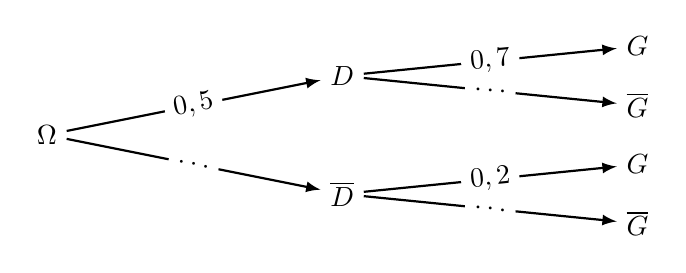
\begin{tikzpicture}[xscale=1,yscale=1]
		\tikzstyle{fleche}=[->,>=latex,thick]
		\tikzstyle{noeud}=[]
		\tikzstyle{feuille}=[]
		\tikzstyle{etiquette}=[midway,sloped,fill=white]
		
		\def\DistanceInterNiveaux{3}
		\def\DistanceInterFeuilles{1}
		
		\def\NiveauA{(0)*\DistanceInterNiveaux}
		\def\NiveauB{(1.25)*\DistanceInterNiveaux}
		\def\NiveauC{(2.5)*\DistanceInterNiveaux}
		\def\InterFeuilles{(-0.75)*\DistanceInterFeuilles}
		
		\node[noeud] (R) at ({\NiveauA},{(1.5)*\InterFeuilles}) {$\Omega$};
		\node[noeud] (Ra) at ({\NiveauB},{(0.5)*\InterFeuilles}) {$D$};
		\node[feuille] (Raa) at ({\NiveauC},{(0)*\InterFeuilles}) {$G$};
		\node[feuille] (Rab) at ({\NiveauC},{(1)*\InterFeuilles}) {$\overline{G}$};
		\node[noeud] (Rb) at ({\NiveauB},{(2.5)*\InterFeuilles}) {$\overline{D}$};
		\node[feuille] (Rba) at ({\NiveauC},{(2)*\InterFeuilles}) {$G$};
		\node[feuille] (Rbb) at ({\NiveauC},{(3)*\InterFeuilles}) {$\overline{G}$};
		
		\draw[fleche] (R)--(Ra) node[etiquette] {${0,5}$};
		\draw[fleche] (Ra)--(Raa) node[etiquette] {${0,7}$};
		\draw[fleche] (Ra)--(Rab) node[etiquette] {$\ldots$};
		\draw[fleche] (R)--(Rb) node[etiquette] {$\ldots$};
		\draw[fleche] (Rb)--(Rba) node[etiquette] {${0,2}$};
		\draw[fleche] (Rb)--(Rbb) node[etiquette] {$\ldots$};
		\end{tikzpicture}
	\end{center}
%
	\begin{enumerate}
		\item Compléter l'arbre de probabilités précédent. 
		\item Calculer la probabilité de l'évènement \og le joueur choisit la console déréglée et il gagne \fg. 
		\item Calculer la probabilité de l'évènement \og le joueur choisit la console non déréglée et il gagne \fg. 
		\item Montrer que la probabilité que le joueur gagne est égale à $0,45$. 
		\item Calculer la probabilité que le joueur ait choisit la console déréglée sachant qu'il a gagné.
	\end{enumerate}
	\item Les événements D et G sont-ils indépendants ? Justifier la réponse.
	%\item Calculer la probabilité de l'événement \og le joueur gagne trois parties de suite \fg{}.
\end{enumerate}

\bigskip

\exonum{1}%\titrexo{Exercice 2}\strut\lignetitre

\medskip

Un nouveau bachelier souhaitant souscrire un prêt automobile pour l'achat de sa première voiture, a le choix entre les trois agences bancaires de sa ville : agence A, agence B et agence C. Après vérification, on a constaté que :
%
\begin{itemize}[topsep=1pt]
	\item 20\:\% des prêts sont souscrits dans l'agence A,
	\item 45\:\% des prêts sont souscrits dans l'agence B,
	\item les autres prêts étant souscrits dans l'agence C. 
\end{itemize}
%
On suppose que tous les clients souscrivent à une assurance dans l'agence où le prêt est souscrit.

Deux types de contrats sont proposés : le contrat tout risque, dit \emph{Zen} et le deuxième contrat appelé \emph{Speed}.

\medskip

\hspace{5mm}80\,\% des clients de l'agence A ayant souscrit un prêt automobile, souscrivent une assurance \emph{Zen}.

\hspace{5mm}30\,\% des clients de l'agence B ayant souscrit un prêt automobile, souscrivent une assurance \emph{Zen}.

\hspace{5mm}$\nicefrac{2}{7}$ des clients de l'agence C ayant souscrit un prêt automobile, souscrivent une assurance \emph{Speed}.

\smallskip 

On interroge au hasard un client d'une de ces trois banques ayant souscrit un contrat d'assurance auto. Soit :
%
\begin{itemize}[topsep=1pt]
	\item[] A : \og le prêt a été souscrit dans l'agence A \fg{},
	\item[] B : \og le prêt a été souscrit dans l'agence B \fg{},
	\item[] C : \og le prêt a été souscrit dans l'agence C \fg{}, 
	\item[] Z : \og le contrat d'assurance \emph{Zen} a été souscrit \fg{}, 
	\item[] S : \og le contrat d'assurance \emph{Speed} a été souscrit \fg{}.
\end{itemize}
%
\begin{enumerate}
	\item  Représenter la situation à l'aide d'un arbre pondéré. 
	\item Déterminer la probabilité que le client interrogé ait souscrit un prêt avec une assurance \emph{Zen} dans l'agence A. 
	\item Vérifier que la probabilité de l'évènement Z est égale à $0,545$. 
	\item Le client a souscrit une assurance \emph{Zen}. Déterminer la probabilité que le prêt soit souscrit dans l'agence C. 
\end{enumerate}

%\bigskip
%
%\titrexo{Exercice 3}\strut\lignetitre
%
%\medskip
%
%\begin{small}
%Un concessionnaire automobile vend deux versions de voitures pour une marque donnée: routière ou break. Pour chaque version il existe deux motorisations : essence ou diesel. Le concessionnaire choisit au hasard un client ayant déjà acheté une voiture. On note : 
%
%\begin{itemize}[topsep=1pt]
%\item[] $R$ l'évènement: \og la voiture achetée est une routière \fg{} ;
%\item[] $B$ l'évènement: \og la voiture achetée est une break \fg{}; 
%\item[] $E$ l'évènement : \og la voiture est achetée avec une motorisation essence \fg{} ; \item[] $D$ l'évènement : \og la voiture est achetée avec une motorisation diesel \fg. 
%\end{itemize}
%
%On sait que :
%
%\begin{itemize}[topsep=1pt]
%\item[$\bullet~$]  65\:\% des clients achètent une voiture routière. 
%\item[$\bullet~$] Lorsqu'un client achète une voiture break, il choisit dans 85\:\% des cas la motorisation diesel. 
%\item[$\bullet~$] 27,3\:\% des clients achètent une voiture routière avec une motorisation diesel.
%\end{itemize}
%\end{small}
%
%\begin{enumerate}
%\item Quelle est la probabilité $p(R)$ de l'événement $R$ ? 
%\item 
%	\begin{enumerate}
%		\item  Construire l'arbre de probabilité complet. 
%	\item  Démontrer que $P_{R}(D) = 0,42$ (probabilité de $D$ sachant $R$). 
%	\end{enumerate}
%\item Calculer $p(D)$. 
%\item Lorsque le concessionnaire a choisi au hasard un client, on note $X$ le prix de vente (en milliers d'euros) de la voiture achetée. Compléter le tableau suivant donnant la loi de probabilité de $X$.
%
%\renewcommand{\arraystretch}{1.3}
%\begin{tabularx}{\linewidth}{|l|*{4}{Y|}}
%	\hline
%	Version &\multicolumn{2}{|c|}{Routière} &\multicolumn{2}{|c|}{Break} \\ \hline
%	Motorisation &Essence&Diesel &Essence &Diesel \\ \hline
%	$x_{i}$ : prix de vente (en milliers d'€) &15 &18 &17 &20\\ \hline 
%	$P_{i}$ : probabilité&& 0,273&&\\ \hline
%\end{tabularx} 
%
%Calculer l'espérance mathématique de $X$. Quelle interprétation peut-on en donner ? 
% 
%\end{enumerate}
%
%\bigskip
%
%\titrexo{Exercice 4}\strut\lignetitre
%
%\medskip
%
%\begin{small}
%Une boîte de chocolats contient 50\,\% de chocolats au lait, 30\,\% de chocolats noirs et 20\,\% de chocolats blancs. Tous les chocolats de la boîte sont de même forme et d'emballage identique. 
%
%Ils sont garnis soit de praliné soit de caramel et, parmi les chocolats au lait, 56\,\% sont garnis de praliné.
% 
%On choisit au hasard un chocolat de la boîte. On suppose que tous les choix sont équiprobables. On note :
% 
%\begin{itemize}[topsep=1pt]
%\item[$\bullet~$] L : l'évènement \og le chocolat choisi est au lait \fg{} ; 
%\item[$\bullet~$] N : l'évènement \og le chocolat choisi est noir \fg{} ; 
%\item[$\bullet~$] B : l'évènement \og le chocolat choisi est blanc \fg{} ; 
%\item[$\bullet~$] A : l'évènement \og le chocolat choisi est garni de praliné \fg{} ; 
%\item[$\bullet~$] $\overline{A}$ : l'évènement \og le chocolat choisi est garni de caramel \fg. 
%\end{itemize}
%\end{small}
%
%\begin{enumerate}
%\item Traduire les données du problème à l'aide d'un arbre de probabilités, qui sera complété au fil des questions. 
%\item Donner la probabilité que le chocolat choisi soit garni de praliné sachant que c'est un chocolat au lait. 
%\item Déterminer la probabilité  que le chocolat choisi soit au lait et garni de praliné. 
%\item Dans la boîte, 21\,\% des chocolats sont noirs et garnis de praliné. 
%
%Montrer que la probabilité que le chocolat choisi soit garni de praliné, sachant que c'est un chocolat noir, est égale à $0,7$. 
%\item Dans la boîte, 60\,\% des chocolats sont garnis de praliné. 
%	\begin{enumerate}
%		\item Déterminer la probabilité que le chocolat choisi soit blanc et garni de praliné. 
%
%		\item En déduire la probabilité que le chocolat choisi soit garni de praliné sachant que c'est un chocolat blanc. 
%	\end{enumerate}
%\item On dispose de deux boîtes de chocolats identiques à celle décrite précédemment. Une personne prend au hasard un chocolat dans la première boîte, puis un chocolat dans la deuxième boîte  (les tirages sont indépendants). 
%
%Déterminer la probabilité de l'évènement : \og l'un des chocolats choisi est garni de praliné et l'autre est garni de caramel \fg. 
%\end{enumerate}

\bigskip

\exonum{2}%\titrexo{Exercice 3}\strut\lignetitre

\medskip

Un site Internet offre la possibilité à des particuliers de vendre des objets aux enchères. Pour chaque objet, la durée des enchères dure une semaine. Si une annonce reçoit une enchère, alors la vente de l'objet est obligatoire à la fin des enchères et ce, même si le vendeur juge le prix de vente trop peu élevé.

Sur ce site une étude statistique a montré que :
\begin{itemize}[]
	\item[$\bullet$] $3/5$ des annonces reçoivent une première enchère le lendemain de leur parution ; dans  ce cas, 75\,\% des vendeurs sont satisfaits du prix de vente final ;
	\item[$\bullet$] $1/3$ des annonces reçoit une première enchère au bout de trois jours et, dans ce cas, 57\,\% des vendeurs sont satisfaits du prix de vente final de leur objet ;
	\item[$\bullet$] les autres annonces ne reçoivent aucune enchère et le vendeur retire alors son objet de la vente. 
\end{itemize}
On choisit au hasard une annonce mise en ligne sur le site. On note :
\begin{itemize}[topsep=1pt]
	\item L : l'évènement \og l'annonce reçoit une première enchère le lendemain de sa parution \fg ; 
	\item T : l'évènement \og  l'annonce reçoit une première enchère au bout de trois jours \fg ; 
	\item A : l'évènement \og l'annonce ne reçoit aucune enchère \fg ; 
	\item S : l'évènement \og le vendeur est satisfait du prix de vente final de son objet \fg ~et $\overline{S}$ son évènement contraire. 
\end{itemize}
%
\begin{enumerate}
	\item Traduire la situation par un arbre de probabilités. 
	\item Calculer la probabilité que l'annonce ait reçu une première enchère le lendemain de sa parution et que le vendeur soit satisfait du prix de vente final. 
	\item Démontrer que la probabilité que le vendeur soit satisfait du prix de vente de son objet est 0,64. 
	\item Un objet est vendu à un prix qui satisfait son vendeur. Quelle est la probabilité que cet objet ait reçu une première enchère dès le lendemain de la parution de l'annonce (le résultat sera donné sous forme décimale, arrondi au centième) ? 
	\item Marc a mis en vente le même jour trois jeux vidéo identiques sur ce site. On suppose que les déroulements des enchères sont indépendants les uns des autres.
	
	Calculer la probabilité qu'à la fin des enchères, Marc soit  satisfait du prix de vente de tous ses jeux vidéo. 
\end{enumerate}

\bigskip

\exonum{3}%\titrexo{Exercice 4}\strut\lignetitre

\medskip

Une boîte de chocolats contient 50\,\% de chocolats au lait, 30\,\% de chocolats noirs et 20\,\% de chocolats blancs. Tous les chocolats de la boîte sont de même forme et d'emballage identique. 

Ils sont garnis soit de praliné soit de caramel et, parmi les chocolats au lait, 56\,\% sont garnis de praliné.
 
On choisit au hasard un chocolat de la boîte. On suppose que tous les choix sont équiprobables. On note :
 %
\begin{itemize}[topsep=1pt]
	\item L : l'évènement \og le chocolat choisi est au lait \fg{} ; 
	\item N : l'évènement \og le chocolat choisi est noir \fg{} ; 
	\item B : l'évènement \og le chocolat choisi est blanc \fg{} ; 
	\item A : l'évènement \og le chocolat choisi est garni de praliné \fg{} ; et $\overline{A}$ :  \og le chocolat choisi est garni de caramel \fg. 
\end{itemize}
%
\begin{enumerate}
	\item Traduire les données du problème à l'aide d'un arbre de probabilités, qui sera complété au fil des questions. 
	\item Donner la probabilité que le chocolat choisi soit garni de praliné sachant que c'est un chocolat au lait. 
	\item Déterminer la probabilité  que le chocolat choisi soit au lait et garni de praliné. 
	\item Dans la boîte, 21\,\% des chocolats sont noirs et garnis de praliné. Montrer que la probabilité que le chocolat choisi soit garni de praliné, sachant que c'est un chocolat noir, est égale à $0,7$. 
	\item Dans la boîte, 60\,\% des chocolats sont garnis de praliné. 
	\begin{enumerate}
		\item Déterminer la probabilité que le chocolat choisi soit blanc et garni de praliné. 

		\item En déduire la probabilité que le chocolat choisi soit garni de praliné sachant que c'est un chocolat blanc. 
	\end{enumerate}
%	\item On dispose de deux boîtes de chocolats identiques à celle décrite précédemment. Une personne prend au hasard un chocolat dans la première boîte, puis un chocolat dans la deuxième boîte (tirages indépendants). 
%
%	Déterminer la probabilité de l'évènement : \og l'un des chocolats choisi est garni de praliné et l'autre est garni de caramel \fg. 
\end{enumerate}
%
%\bigskip
%
%\begin{center}
%\includegraphics[scale=0.20]{graphics/chap04_exos_humour.eps} 
%
%{\scriptsize \textit{Le Devin}, Uderzo \& Goscinny}
%\end{center}
\end{document}